%%
%% Author: dariochinelli
%% 2021-04-05
%%


\section{Onde di Materia}
\subsection{Ipotesi di De Broglie}
Venne introdotto questo concetto nel 1924 nella tesi di dottorato di Louis De Broglie.
Le equazioni per la radiazione elettromagnetica 
\begin{equation}
E = h\nu \quad \quad p = \frac{ h}{\lambda }
\end{equation}
che descrivono l'energia e la quantità di moto sono valide anche per le particelle.
Da cui si ricava la \textbf{Lunghezza d'onda di De Broglie}
\begin{equation}
\lambda = \frac{ h}{p }
\end{equation}

\paragraph{Esempio}
Qual è la lunghezza d'onda di De Broglie di una palla di massa $ m =\SI{1}{kg}$ che si muove a una velocità $v = \SI{10}{m/s}$?
Soluzione:
\begin{equation}
\lambda = \frac{ h}{p } = \frac{ h}{m v } = \frac{ \SI{6.6e-34}{j.s}}{\SI{1}{kg} . \SI{10}{m/s} } = \SI{6.6e-35}{m} = \SI{6.6e-25}{\AA}
\end{equation}
Qual è la lunghezza d'onda di De Broglie di un elettrone avente energia cinetica \SI{100}{eV}?
\begin{equation}
\begin{split}
\lambda & = \frac{ h}{p } = \frac{ h}{\sqrt{2mK} } 
= \frac{\SI{6.6e-34}{j.s} }{\sqrt{ 2 \cdot \SI{9.1e-31}{kg} \cdot \SI{100}{eV} \cdot \SI{1.6e-19}{j / eV} } } \\
& = \frac{ \SI{6.6e-34}{j.s}}{\SI{5.4e-24}{kg.m/s} } = \SI{1.2e-10}{m} = \SI{1.2}{\AA}
\end{split}
\end{equation}

Da questi conti si vede quanto sia difficilmente osservabile la lunghezza d'onda di un oggetto macroscopico, che differisce da quella di un elettrone come in esempio di un fattore \SI{e-25}{}.
Dagli esperimenti di ottica si vede che la natura ondulatoria della luce si manifesta solo quando le grandezze in gioco sono confrontabili con la lunghezza d'onda della radiazione esaminata.
I cristalli, ad esempio, hanno una struttura la cui distanza inter-atomica è di una grandezza confrontabile con quella della lunghezza d'onda di un fascio di fotoni X, vedi legge di Bragg.
Una cosa analoga avviene con le onde di materia, potrò allora rivelare la natura ondulatoria di un elettrone solo se interagirà con qualcosa della dimensione dell'ordine dell'Amstrong, come visto sopra.
Non potrò vedere la natura ondulatoria della palla da $\SI{1}{kg}$ poiché non c'è niente in natura della dimensione di $\SI{e-25}{\AA}$ che possa far interferire questo oggetto.



\subsection{Esperimento di Davisson e Germer}
\paragraph{Apparato sperimentale} 
Facendo riferimento alla figura \ref{app_spe}: si ha un filamento di Tungsteno $(F)$ riscaldato che emette elettroni, i quali vengono accelerati, grazie ad una differenza di potenziale $(V)$, e fatti incidere su un bersaglio cristallino di Nichel $(C)$.
Ad un angolo $\theta$ viene posizionato un detector $(D)$, dove l'angolo può esser fatto variare per osservarne la diffusione.

\begin{figure}[h]
\centering
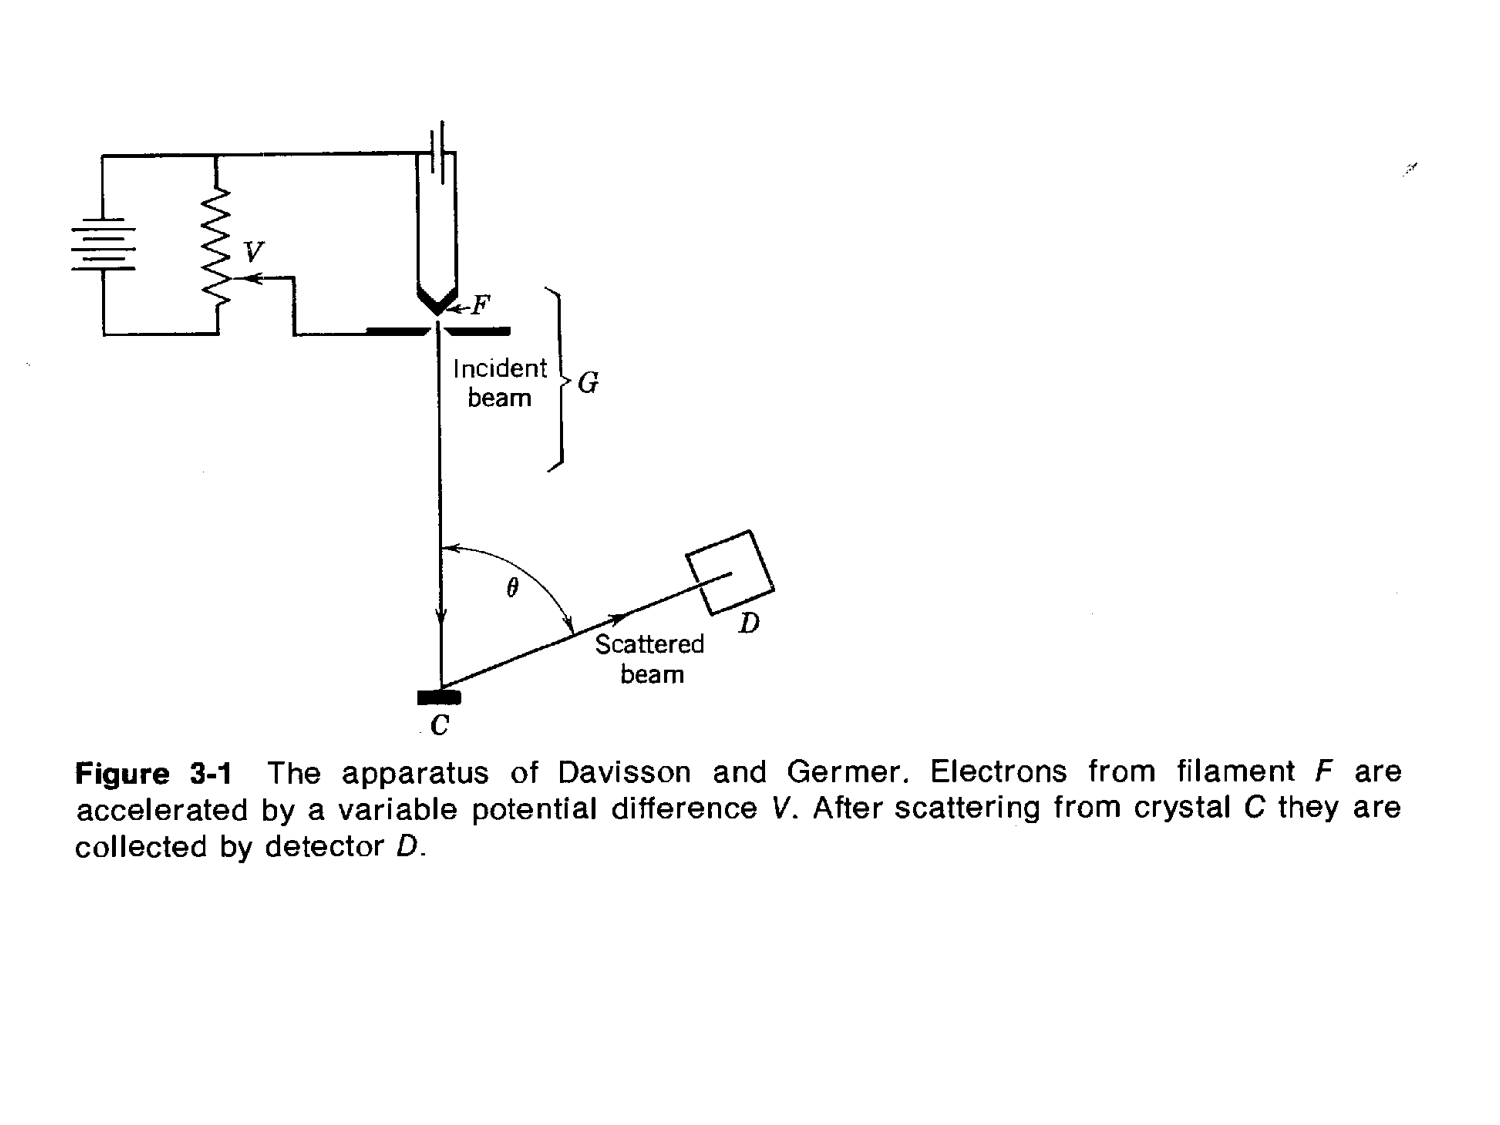
\includegraphics[scale=0.5]{/esp_devissongermer}
\caption{Schema della strumentazione utilizzata}
\label{app_spe}
\end{figure}
\begin{figure}[h]
\centering
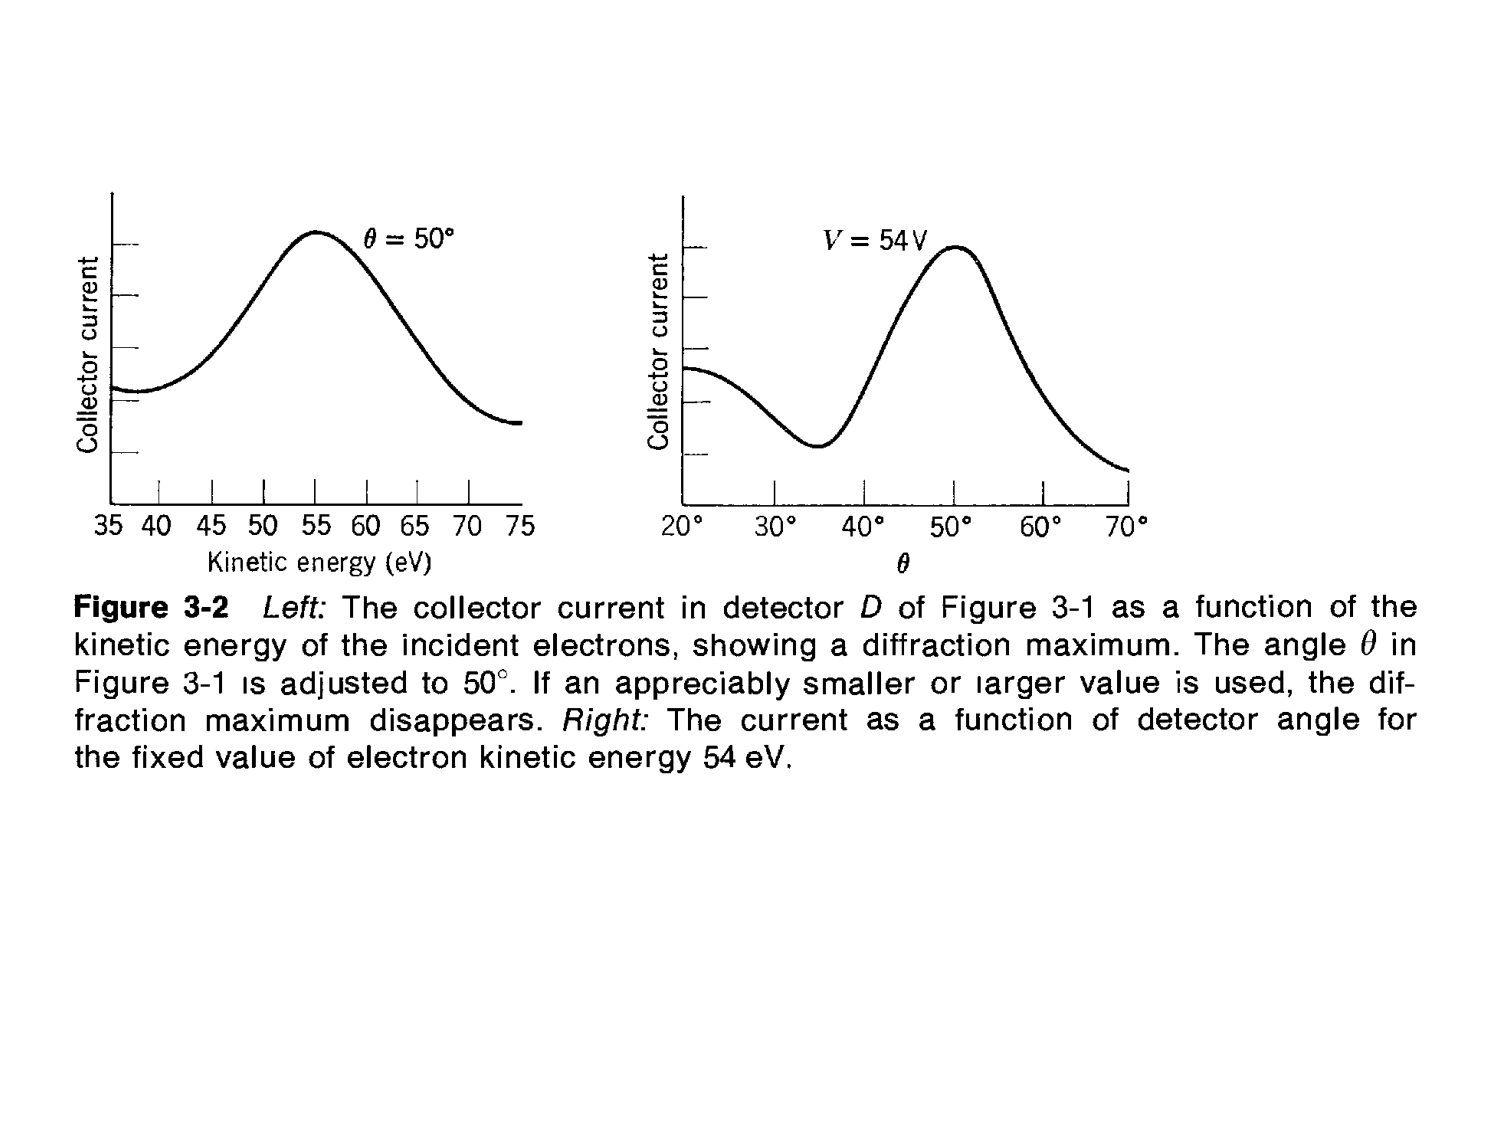
\includegraphics[scale=0.5]{/ris_esp_devissongermer}
\caption{Risultati sperimentali}
\label{res_spe}
\end{figure}

\paragraph{Risultati sperimentali}
Variando l'angolo di osservazione ed il potenziale applicato, quindi l'energia degli elettroni incidenti, osservarono gli andamenti evidenziati in figura \ref{res_spe} e notarono un picco nel segnale, quindi nell'intensità e quindi nel numero di elettroni diffusi per unità di tempo, in corrispondenza di un angolo $\theta = 50^{\circ}$.
Allo stesso modo fissando il potenziale a $V = \SI{54}{V}$ e facendo variare l'angolo, videro un picco in corrispondenza dell'angolo $\theta = 50^{\circ}$.
Con questa doppia misura i risultati si confermano reciprocamente.

\paragraph{Conclusioni}
Questo fenomeno non è spiegabile considerando l'elettrone come una particella.
Utilizzando una interpretazione ondulatoria del fascio di elettroni questo risultato lo si descrive come un fenomeno di interferenza:
i picchi risultano derivare dall'interferenza della particella-onda elettrone che attraversa la struttura cristallina.

Lo stesso fenomeno avviene anche utilizzando un fascio di elettroni molto debole, al punto da ipotizzare che solo un elettrone per volta attraversasse il cristallo, in modo quindi da escludere una interazione fra più elettroni e dimostrare che ogni singolo elettrone interferisce come onda.

Solo pochi anni prima era stata resa nota l'ipotesi di De Broglie, infatti Davisson e Germer individuarono questo fenomeno involontariamente, nemmeno ne erano al corrente.
Il loro scopo era far incidere gli elettroni sul campione di Nichel per acquisire informazioni sulla superficie di questo oggetto.
Fu Davisson che, dopo aver partecipato ad una conferenza sull'ipotesi di De Broglie, si accorse che c'era un collegamento tra il loro esperimento e tale ipotesi.

\paragraph{Teorie a confronto}
Considerando l'ipotesi di De Broglie, posso calcolare la lunghezza d'onda di De Broglie dell'elettrone nell'esperimento di Davisson e Germer
\begin{equation}
\lambda = \frac{ h}{p } = \frac{ h}{\sqrt{2mK} } 
= \frac{\SI{6.6e-34}{j.s} }{\sqrt{ 2 \cdot \SI{9.1e-31}{kg} \cdot \SI{54}{eV} \cdot \SI{1.6e-19}{j / eV} } } 
= \SI{1.67e-10}{m} = \SI{1.67}{\AA}
\end{equation}
Ed invece calcolando la lunghezza d'onda considerando la legge di Bragg trovo
\begin{equation}
\begin{split}
& 2 d \sin \varphi = n \lambda \\
& \lambda = 2 d \sin \varphi = 1.65 \AA
\end{split}
\end{equation}
trovo quindi un accordo molto buono tra le due teorie.





\subsection{Principio di complementarietà di Neils Bohr}
I modelli ondulatori e corpuscolari sono complementari: se una misura rivela il carattere ondulatorio allora nella stessa misura è impossibile determinarne il carattere corpuscolare, in un esperimento è quindi possibile osservare o la natura ondulatoria o la natura corpuscolare.

\paragraph{Ad esempio} nell'esperimento di Compton viene messa in evidenza la doppia natura, si utilizza uno stesso apparato ma è come se fossero due esperimenti in cascata in cui il primo, l'interazione della radiazione X con il target di carbonio, evidenzia la natura corpuscolare ed il secondo, in cui si osserva la diffrazione alla Bragg, quella ondulatoria.
Non c'è contraddizione con la complementarietà di Bohr perché non è un unico esperimento ma sono due esperimenti in cascata.


\paragraph{L'interpretazione probabilistica} è ciò che viene utilizzata per conciliare le due nature della radiazione e delle onde

\begin{equation}
\begin{split}
E & = A \sin \Bigl[ 2\pi \Bigl(  \frac{ x}{\lambda } - \nu t  \Bigr) \Bigr] \quad \mbox{Onda di radiazione} \\
\Psi & = A \sin \Bigl[ 2\pi \Bigl(  \frac{ x}{\lambda } - \nu t  \Bigr) \Bigr] \quad \mbox{Onda di materia}
\end{split}
\end{equation}

Il quadrato della funzione d'onda media descrive la \textbf{probabilità} di trovare una particella in un punto dello spazio in un certo momento.

Interpretazione nata dalla "Scuola di Copenhagen": quindi Heisenberg, Bohr, Born ...
si è imposta questo tipo di trattazione probabilistica, dopo varie discussioni e dibattiti.


 








